\section{\review{Resonances}}


%----------------------------------------
%             Tune Diagram
%----------------------------------------
\subsection{\review{Tune Diagram}}

The resonances discussed in this thesis are related to the optics of the accelerator.
Such resonances create unstable motion and can lead to loosing particles.

\begin{figure}[!htb]
    \centering
    \begin{subfigure}[b]{0.6\textwidth}
        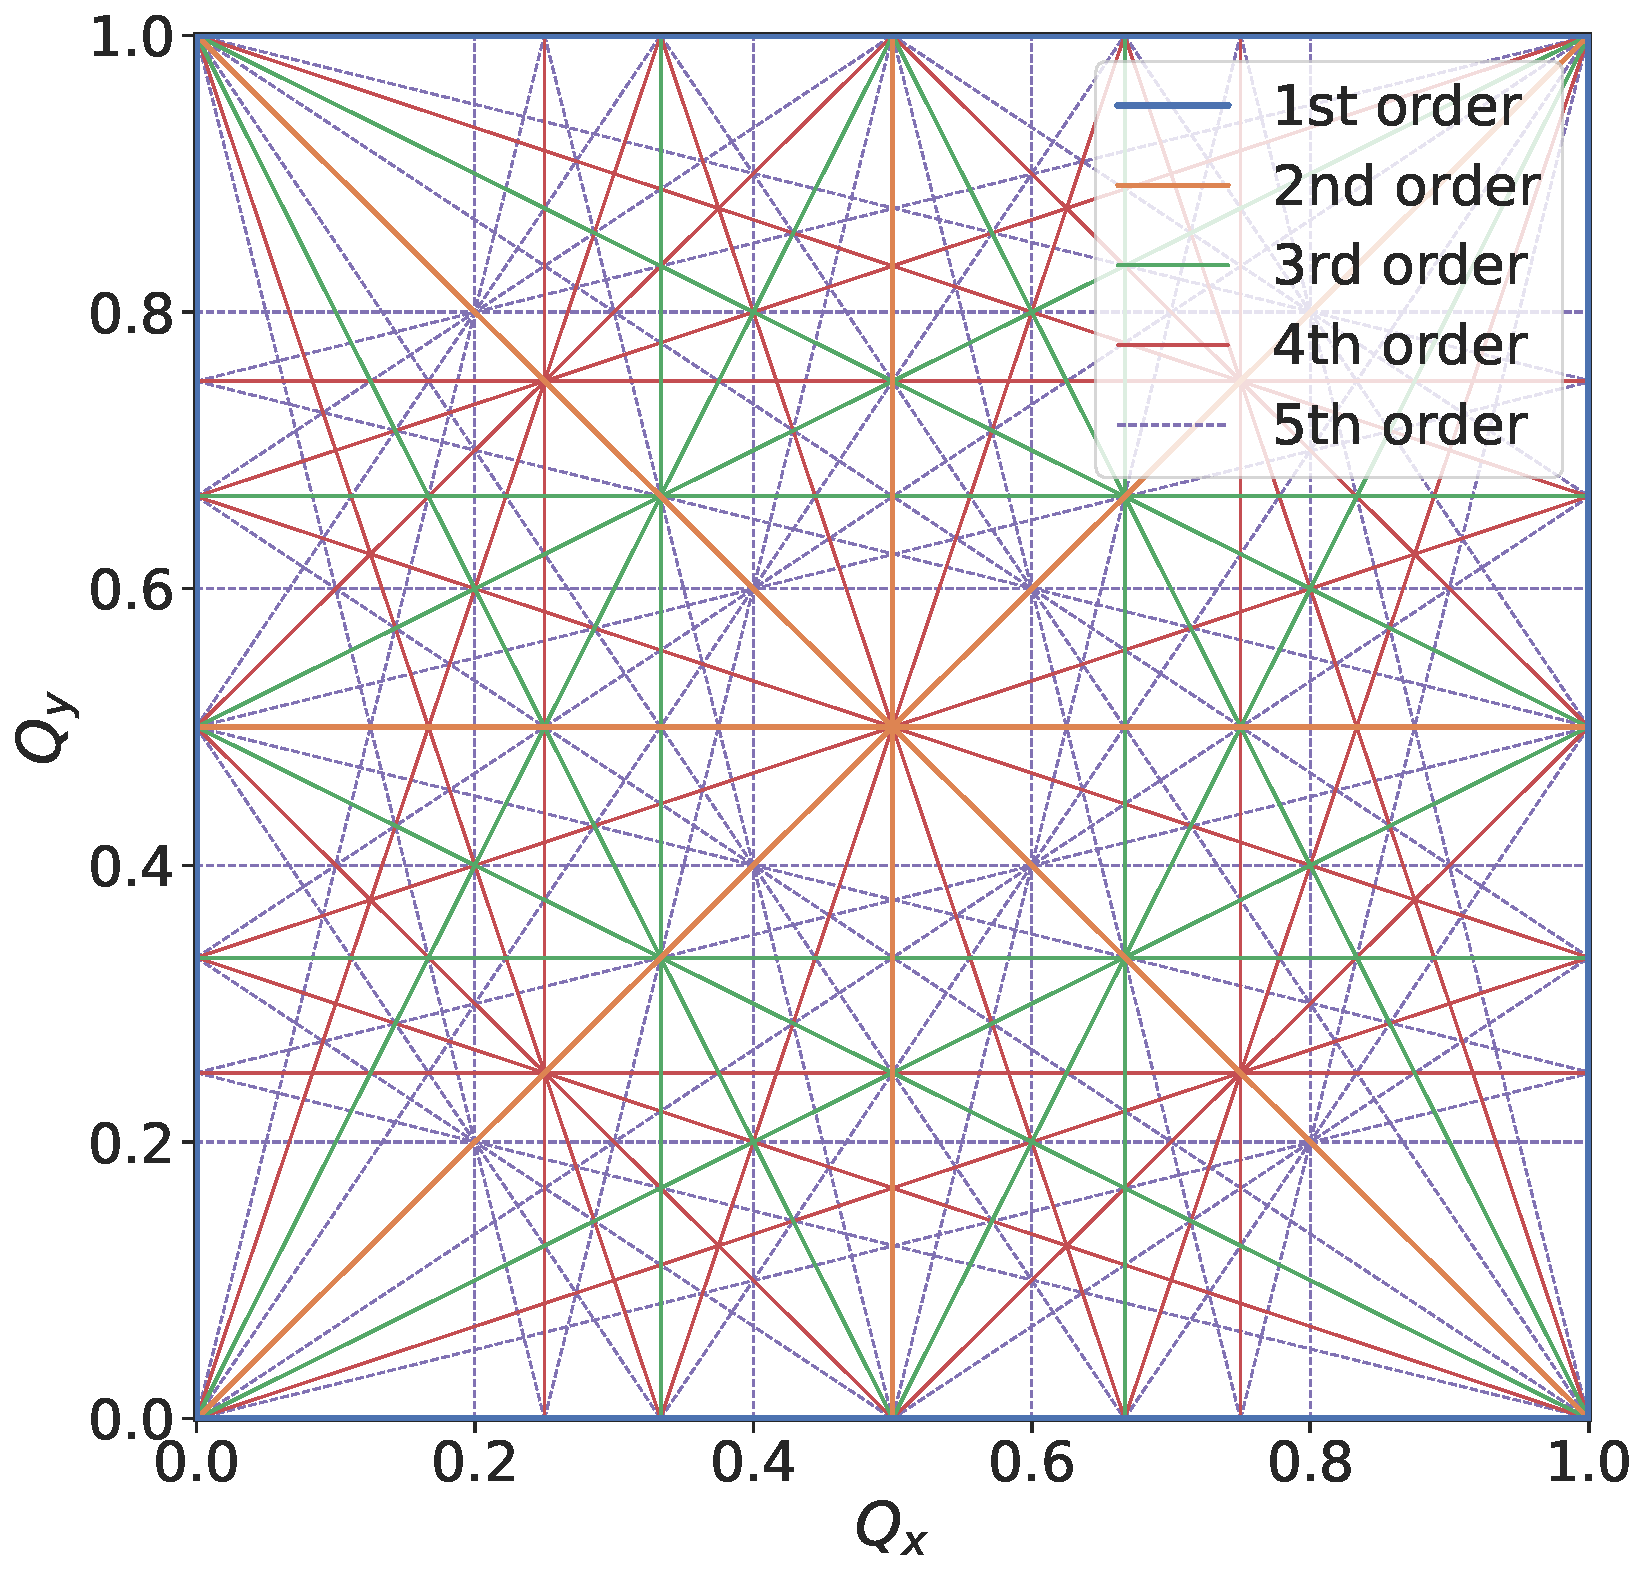
\includegraphics[width=1\textwidth]{images/resonance_diagram_n5.pdf}
        \caption{Resonances lines up to decapoles ($n \leq 5$).}
        \label{fig:resonances:diagram_n5}
    \end{subfigure}
    \\
    \begin{subfigure}[b]{0.6\textwidth}
        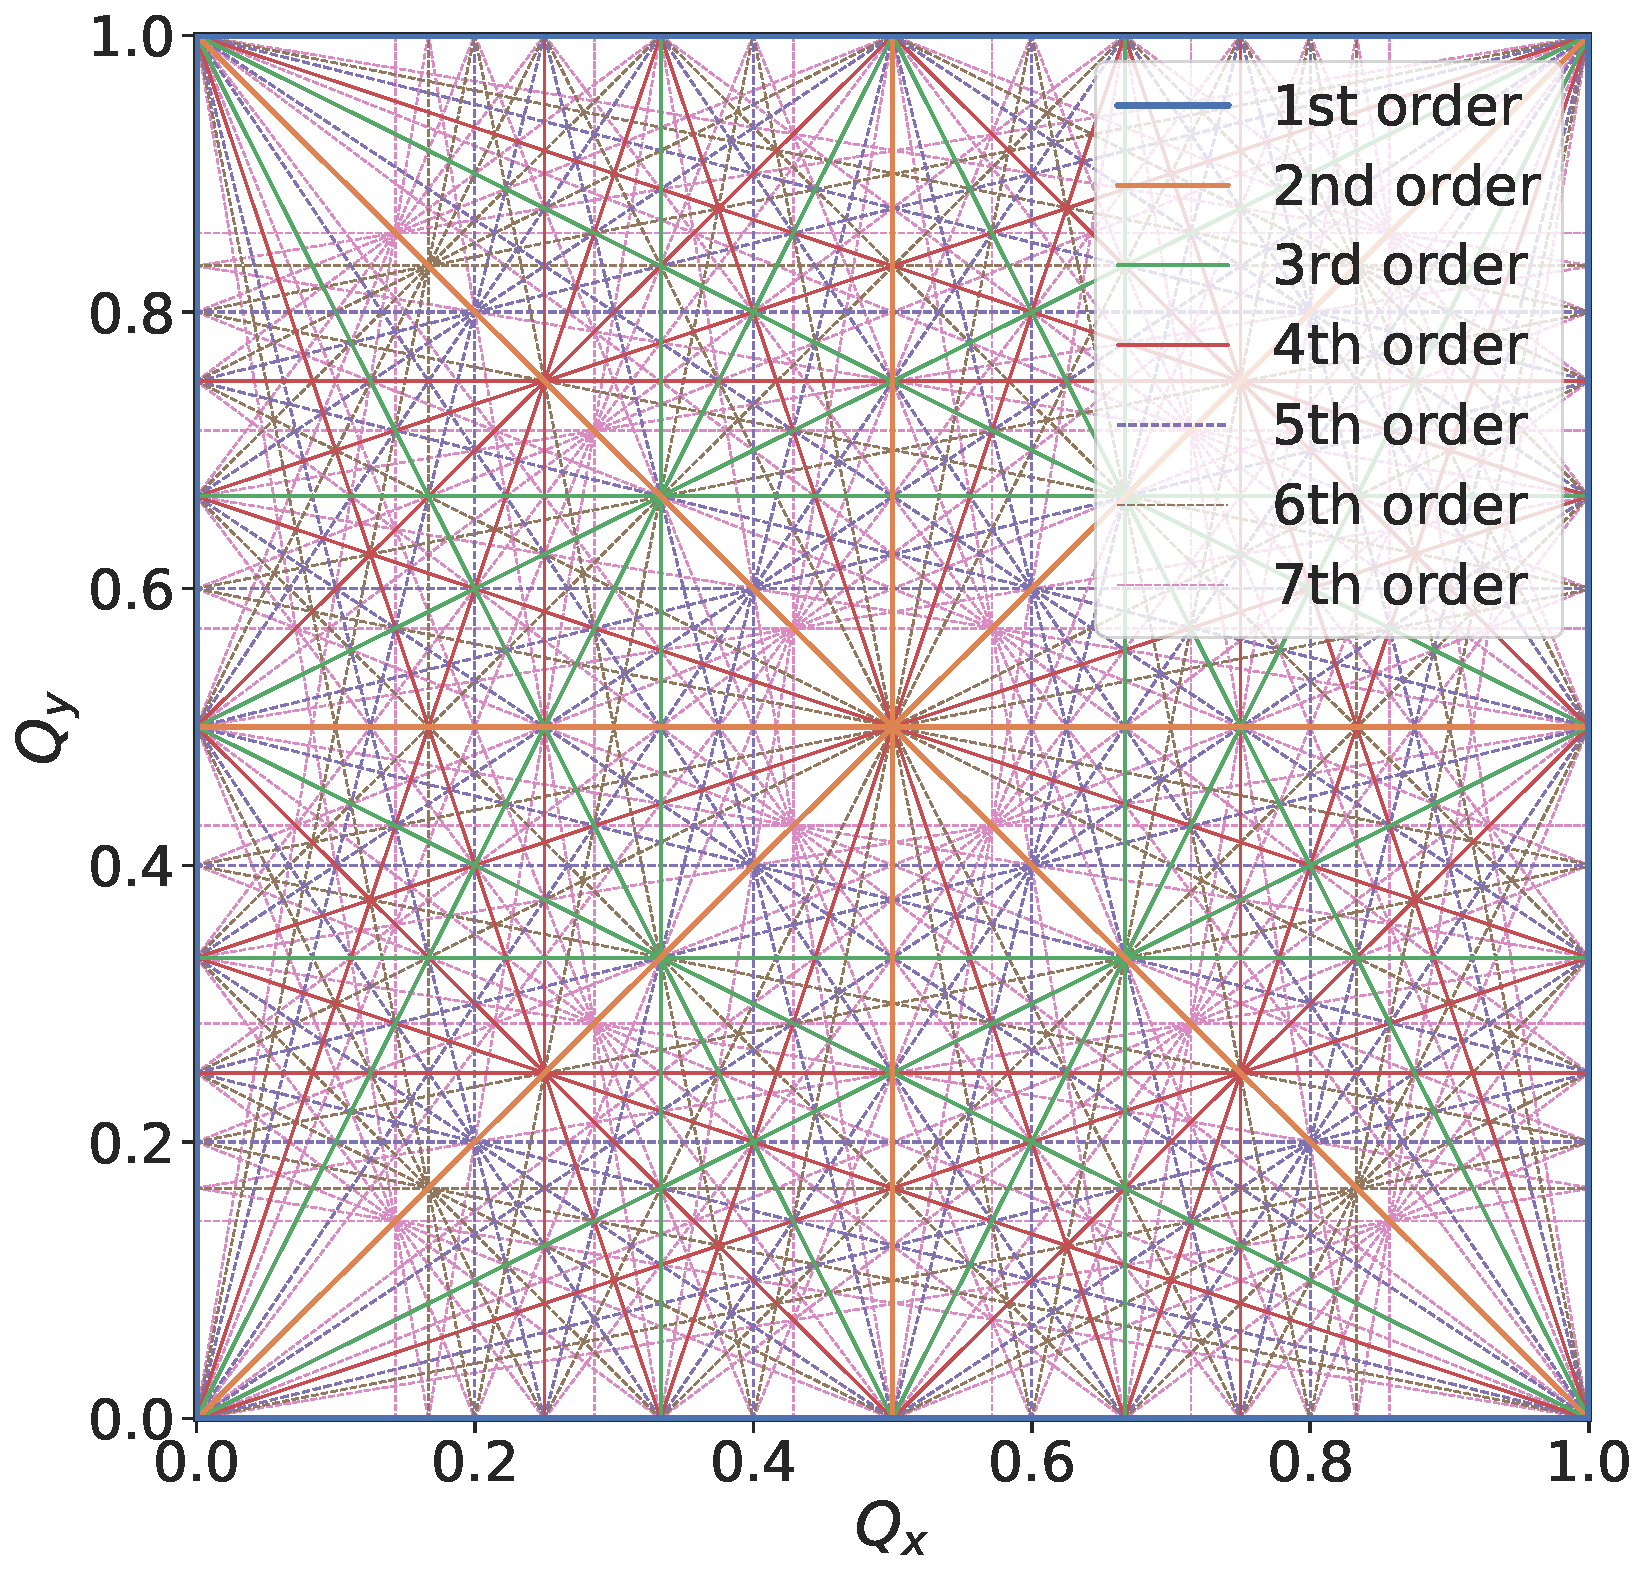
\includegraphics[width=\textwidth]{images/resonance_diagram_n7.pdf}
        \caption{Resonances lines up to decatetrapole ($n \leq 7$).}
        \label{fig:resonances:diagram_n7}
    \end{subfigure}
    \caption{Tune diagram with resonance lines excited by different multipole orders. The working
    point is chosen in an area where few lines are present. When considering higher orders, it
    becomes apparent that the beam will inevitably hit several resonances.}
    \label{fig:resonances:diagrams}
\end{figure}

\Cref{fig:resonances:diagram_n5} shows a tune diagram where the fractional part of tunes $Q_x$ and
$Q_y$ can be related to resonance lines excited by multipoles up to decapoles ($n=5$).
It becomes apparent that the diagram fills quickly when considering further orders, as shows
\cref{fig:resonances:diagram_n7}.  Thankfully, the higher the multipole order, the weaker the
resonances usually are. This makes choosing a working point possible, even if some particles are
hitting resonance lines.



When considering the resonance driving terms $f_{jklm}$ from \cref{eq:coordinate_systems:fjklm}, it
can be noted that the term diverges for particular tune values. This leads to a disproportionate
increase in particles position in phase-space, eventually leading to loosing them.
Resonant conditions due to the tunes can thus be described by the following condition:

\begin{equation}
    (j-k)Q_x + (l-m)Q_y = p \quad,\quad j,k,l,m,p \in \mathcal{Z}.
\end{equation}

\FloatBarrier


%----------------------------------------
%          Frequency Spectrum
%----------------------------------------
\subsection{\review{Frequency Spectrum}}
\label{section:background:frequency_spectrum}

As seen in \cref{eq:coordinate_systems:linear_position_normal_form}, resonance driving terms have an
impact on the transverse motion of a particle. This means that performing a FFT on the turn-by-turn
signal will reveal spectral lines linked to specific resonance driving terms.
Each RDT $f_{jklm}$ can thus be observed in either one or both the frequency spectrums of the
horizontal and vertical planes, at multiples of $Q_x \pm Q_y$. \Cref{eq:resonances:rdt_spectrum}
shows where those lines would appear:

\begin{equation}
    \begin{aligned}
    & H_{jklm} \;&&\text{at}\; (1 - j + k)Q_x + (m - l)Q_y \quad&&; \quad j \ne 0 \\
    & V_{jklm}   &&\text{at}\; (k - j)Q_x + (1 - l + m)Q_y      &&; \quad l \ne 0.
    \end{aligned}
    \label{eq:resonances:rdt_spectrum}
\end{equation}

The RDT $f_{3000}$ coming from sextupoles can for example be seen in the horizontal spectrum at
$(1-3+0)Q_x + (0-0)Q_y = -2Q_x$. For a value $Q_x = 0.27$, the line is seen at $0.46$. No line can
be seen in the vertical spectrum due to $l = 0$. Detailed tables of such lines for RDTs up to order
6 can be found in \cref{appendix:rdts}.

The amplitude of each line will depend on the action $I_z$ and the amplitude of the
RDT~\cite{bartolini_normal_1997}:

\begin{equation}
    \begin{aligned}
    |H_{f_{jklm}}| &= 2 j (2 I_x)^\frac{j+k-1}{2} (2 I_y)^\frac{l+m}{2} |f_{jklm}| \\
    |V_{f_{jklm}}| &= 2 l (2 I_x)^\frac{j+k}{2} (2 I_y)^\frac{l+m-1}{2} |f_{jklm}|.
    \end{aligned}
    \label{eq:resonances:amplitude_line}
\end{equation}


%                 RDTs
%----------------------------------------
\paragraph{\review{Resonance Driving Terms}}

By reworking the previous \cref{eq:resonances:amplitude_line}, it can be seen that RDTs are factors
of the line amplitude and the actions $I_x$ and $I_z$:

\begin{equation}
    \begin{aligned}
    |f_{jklm}| &= \frac{|H_{f_{jklm}}|}{2 j (2 I_x)^\frac{j+k-1}{2} (2 I_y)^\frac{l+m}{2}} \\
    |f_{jklm}| &= \frac{|V_{f_{jklm}}|}{2 l (2 I_x)^\frac{j+k}{2} (2 I_y)^\frac{l+m-1}{2}} .
    \label{eq:resonances:amplitude_rdt}
    \end{aligned}
\end{equation}

In practice, an approximation of $J = I$ is done. The RDT is then related to the fit of the line
amplitude versus the action.% as shown in \cref{fig:resonances:fit_rdt}.

%\begin{figure}[H]
%    \centering
%    \includegraphics[width=0.8\textwidth]{example-image-a}
%    \caption{.}
%    \label{fig:resonances:fit_rdt}
%\end{figure}